\section{Langkah-Langkah Percobaan}
 
\subsection{Konfigurasi Wireless Point to Point}
\begin{enumerate}
    \item \textbf{Reset Router} \\
    Pastikan router dalam kondisi default (tanpa konfigurasi sebelumnya). Lakukan reset melalui Winbox: \texttt{System} $\rightarrow$ \texttt{Reset Configuration}, kemudian centang \texttt{No Default Configuration}.
    
    \item \textbf{Login ke Router} \\
    Gunakan aplikasi Winbox untuk masuk ke router menggunakan MAC address atau IP default. Masuk sebagai \texttt{admin} tanpa password jika belum diatur.

    \item \textbf{Aktivasi Interface Wireless Wlan1} \\
    Akses menu \texttt{Wireless}, aktifkan interface \texttt{wlan1}. Pada Router A, atur \texttt{Mode: Bridge}, \texttt{SSID: PointToPoint\_NoKelompok}. \\
    Pada Router B, atur \texttt{Mode: Station}, lalu gunakan tombol \texttt{Scan}, pilih jaringan dengan SSID sesuai Router A, lalu klik \texttt{Connect}.

    \item \textbf{Konfigurasi IP Address pada Wlan1} \\
    Atur IP pada interface wlan1 sebagai jalur komunikasi antar router. \\
    Router A: \texttt{10.10.10.1/29} \\
    Router B: \texttt{10.10.10.2/29}

    \item \textbf{IP LAN via Ether2} \\
    Tambahkan IP pada interface \texttt{ether2} yang terhubung ke laptop. \\
    Router A: \texttt{192.168.20.1/24} \\
    Router B: \texttt{192.168.30.1/24}

    \item \textbf{Routing Statis} \\
    Tambahkan routing manual dari menu \texttt{IP $\rightarrow$ Routes}. \\
    Router A: \texttt{Dst Address: 192.168.30.0/24, Gateway: 10.10.10.2} \\
    Router B: \texttt{Dst Address: 192.168.20.0/24, Gateway: 10.10.10.1}

    \item \textbf{Uji Koneksi Router} \\
    Ping dari Router A ke B: \texttt{ping 10.10.10.2} \\
    Ping dari Router B ke A: \texttt{ping 10.10.10.1}

    \item \textbf{Pengaturan IP Statis di Laptop} \\
    Laptop Router A: IP \texttt{192.168.20.2}, Gateway \texttt{192.168.20.1} \\
    Laptop Router B: IP \texttt{192.168.30.2}, Gateway \texttt{192.168.30.1}

    \item \textbf{Tes Koneksi Antar Laptop} \\
    Uji koneksi dari laptop yang terhubung ke Router A menuju laptop di Router B menggunakan perintah \texttt{ping}.
\end{enumerate}

\subsection{Konfigurasi Wireless Point to Multipoint}
\begin{enumerate}
    \item Lakukan reset konfigurasi router seperti langkah sebelumnya.
    
    \item Login ke router menggunakan Winbox dan masuk sebagai user admin.
    
    \item Aktifkan interface \texttt{wlan1} melalui menu \texttt{Wireless}. \\
    Router A: \texttt{Mode: AP Bridge}, \texttt{SSID: PointToMultipoint\_NoKelompok} \\
    Router B: \texttt{Mode: Station Bridge}, lalu scan dan sambungkan ke SSID milik Router A.
    
    \item Tambahkan IP address untuk \texttt{wlan1}. \\
    Router A: \texttt{10.10.10.1/29} \\
    Router B: \texttt{10.10.10.2/29}

    \item Tambahkan IP pada interface \texttt{ether2}. \\
    Router A: \texttt{192.168.20.1/24} \\
    Router B: \texttt{192.168.30.1/24}

    \item Tambahkan routing manual. \\
    Router A: \texttt{Dst: 192.168.30.0/24, Gateway: 10.10.10.2} \\
    Router B: \texttt{Dst: 192.168.20.0/24, Gateway: 10.10.10.1}

    \item Uji koneksi antar router menggunakan ping.

    \item Atur IP statis di laptop yang terhubung ke masing-masing router. \\
    Laptop A: IP \texttt{192.168.20.2}, Gateway \texttt{192.168.20.1} \\
    Laptop B: IP \texttt{192.168.30.2}, Gateway \texttt{192.168.30.1}

    \item Uji konektivitas antar laptop.
\end{enumerate}

\subsection{Konfigurasi Wireless Bridge}
\begin{enumerate}
    \item Lakukan reset konfigurasi router agar bersih dari pengaturan lama.

    \item Login ke router menggunakan Winbox.

    \item Aktifkan \texttt{wlan1} dan atur konfigurasi: \\
    Router A: \texttt{Mode: Bridge}, SSID: \texttt{WirelessBridge\_NoKelompok} \\
    Router B: \texttt{Mode: Station Pseudobridge}, sambungkan ke SSID Router A.

    \item Atur IP untuk interface \texttt{wlan1}. \\
    Router A: \texttt{10.10.10.1/29} \\
    Router B: \texttt{10.10.10.2/29}

    \item Atur IP untuk interface \texttt{ether2}. \\
    Router A: \texttt{192.168.10.2/24} \\
    Router B: \texttt{192.168.10.3/24}

    \item Tambahkan \texttt{bridge} untuk menggabungkan interface \texttt{wlan1} dan \texttt{ether2}. \\
    Masuk ke menu \texttt{Bridge} $\rightarrow$ buat bridge baru (misal: bridge1), lalu tambahkan port: \texttt{wlan1} dan \texttt{ether2} ke dalam bridge tersebut.

    \item Lakukan uji koneksi antar router menggunakan ping.

    \item Atur IP statis di laptop: \\
    Laptop A: IP \texttt{192.168.10.5}, Gateway \texttt{192.168.10.2} \\
    Laptop B: IP \texttt{192.168.10.7}, Gateway \texttt{192.168.10.3}

    \item Lakukan ping antar laptop untuk memastikan konektivitas berhasil.
\end{enumerate}

\section{Analisis Hasil Percobaan} 
Konfigurasi Point to Point berhasil dilakukan dengan Router A sebagai Bridge dan Router B sebagai Station. Hasil uji koneksi antar router dan laptop menunjukkan komunikasi berjalan lancar dengan IP dan routing statis yang tepat. Keberhasilan ping antar laptop membuktikan jalur komunikasi antar jaringan berfungsi baik. Hambatan yang mungkin muncul berasal dari kesalahan konfigurasi IP, mode interface, atau gangguan sinyal wireless.
 
Pada skenario Point to Multipoint, Router A berfungsi sebagai AP dan Router B sebagai Station Bridge. Koneksi wireless berhasil dibangun, dan dengan konfigurasi IP serta routing yang sesuai, komunikasi antar laptop dapat dilakukan tanpa masalah. Topologi ini efektif untuk membangun jaringan terpusat, namun tetap bergantung pada ketelitian dalam pengisian IP dan pemilihan SSID yang tepat.
 
Wireless Bridge memungkinkan dua jaringan LAN digabungkan menjadi satu melalui koneksi wireless. Dengan menggabungkan \texttt{wlan1} dan \texttt{ether2} ke dalam bridge interface, komunikasi antar laptop dalam satu subnet berhasil dilakukan tanpa perlu routing tambahan. Keberhasilan konfigurasi ini sangat bergantung pada penggabungan interface yang benar dan mode wireless yang sesuai.


\section{Hasil Tugas Modul}
\begin{figure}[H]
\centering

\includegraphics[width=0.8\textwidth]{P1/img/1.png}
    \end{figure}

    \section{Kesimpulan}
Berdasarkan hasil praktikum yang telah dilakukan, dapat disimpulkan bahwa konfigurasi jaringan wireless menggunakan perangkat MikroTik dapat dilakukan dengan berbagai topologi seperti Point to Point, Point to Multipoint, dan Wireless Bridge. Setiap metode memiliki karakteristik dan keunggulan tersendiri dalam hal komunikasi dan struktur jaringan. Pada konfigurasi Point to Point, komunikasi antar dua router dapat berjalan stabil dengan pengaturan IP dan routing statis yang benar. Sementara itu, Point to Multipoint memungkinkan satu router pusat melayani beberapa client, cocok untuk topologi jaringan terpusat. Wireless Bridge menunjukkan bahwa dua jaringan lokal dapat digabungkan menjadi satu subnet tanpa perlu routing tambahan, cukup dengan bridge interface. Keberhasilan praktikum sangat bergantung pada ketelitian dalam melakukan konfigurasi, mulai dari pengaturan mode wireless, IP address, hingga routing dan bridge. Praktikum ini memberikan pemahaman langsung mengenai konsep dasar jaringan wireless serta penerapannya dalam membangun infrastruktur jaringan yang efektif dan efisien.


\section{Lampiran}
\subsection{Dokumentasi saat praktikum}
\begin{figure}[H]
    \centering
    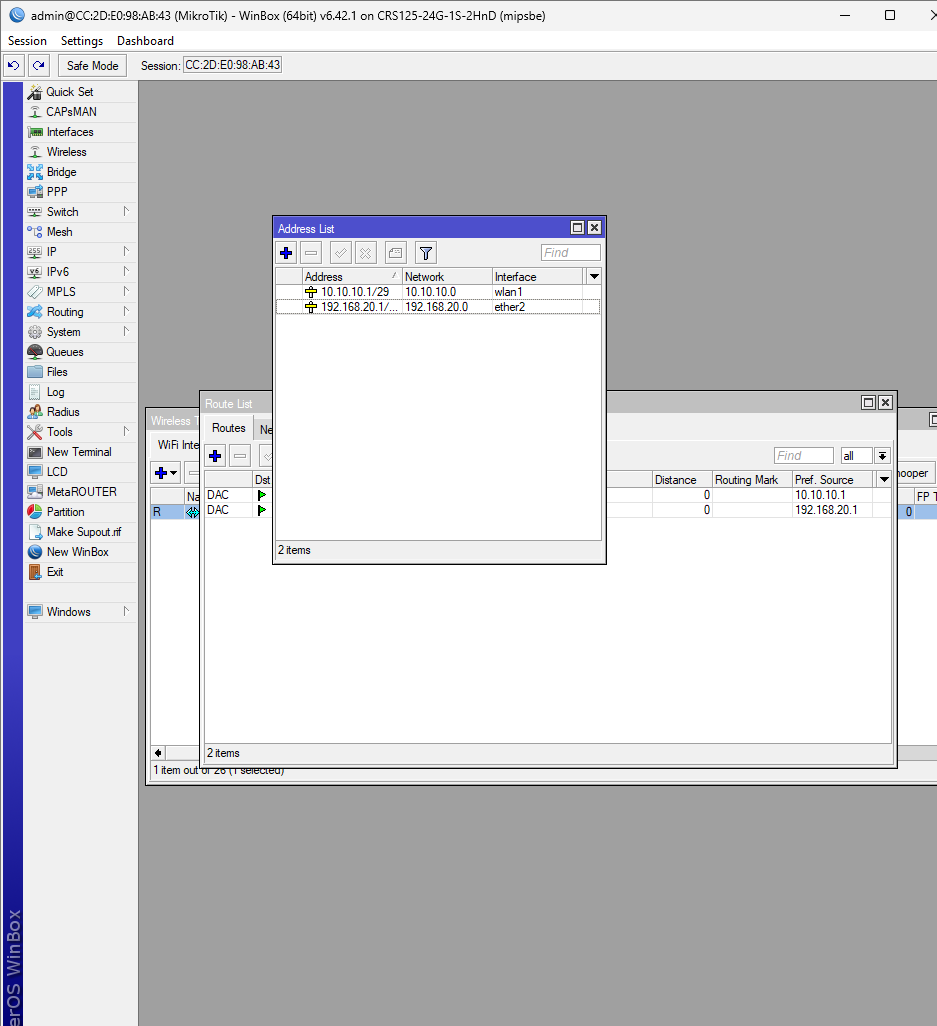
\includegraphics[width=0.8\textwidth]{P1/img/2.png}
\end{figure}
\begin{figure}[H]
    \centering
    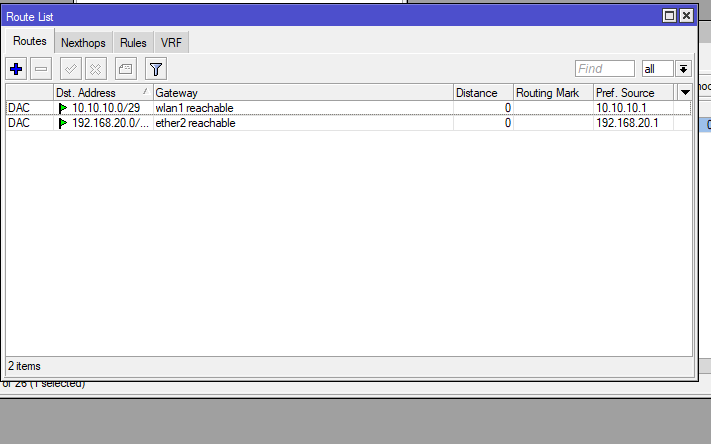
\includegraphics[width=0.8\textwidth]{P1/img/3.png}
\end{figure}
\begin{figure}[H]
    \centering
    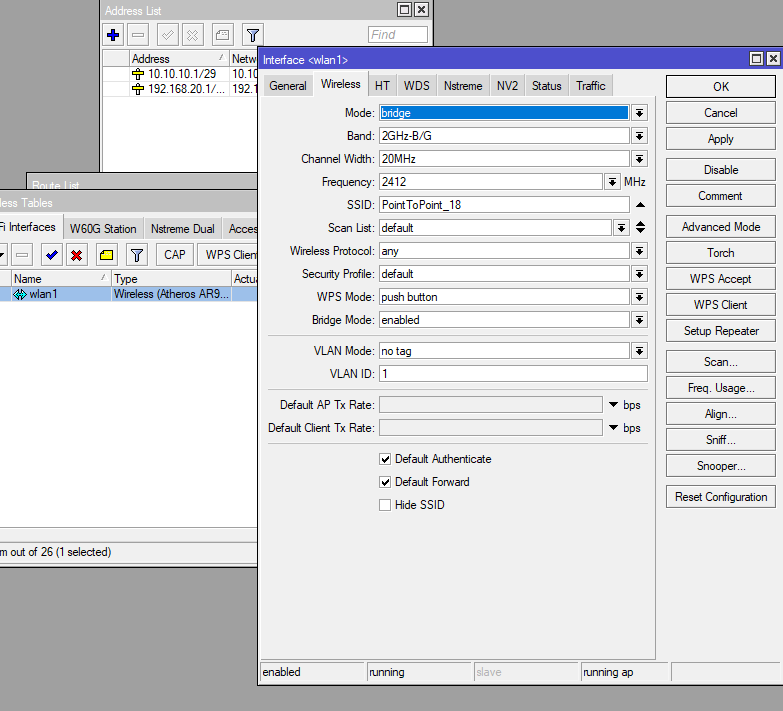
\includegraphics[width=0.8\textwidth]{P1/img/4.png}
\end{figure}
\begin{figure}[H]
    \centering
    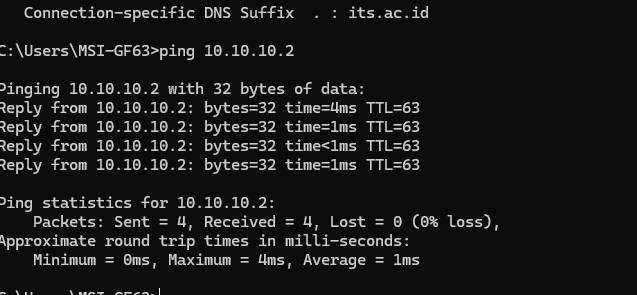
\includegraphics[width=0.8\textwidth]{P1/img/5.png}
\end{figure}
\begin{figure}[H]
    \centering
    
\includegraphics[width=0.8\textwidth]{P1/img/6.png}
\end{figure}